\documentclass[a4paper,10pt]{article}
\usepackage{graphicx}
\usepackage{ucs}
\usepackage[utf8x]{inputenc} %instalar latex-ucs.
\usepackage[spanish]{babel}
\usepackage{listings}
\usepackage[colorlinks=true]{hyperref}

% Title Page
\title{ADT\_rovioAPI\\Interfaz de aplicación de código abierto en C++  para el control de Rovio™ - WowWee®}
\author{Mario Chririnos Colunga\\ Áurea - Desarrollo Tecnológico}


\begin{document}
\maketitle

% \begin{abstract}
% 
% \end{abstract}

\tableofcontents
\section{Introducción}

Este documento está estructurado de la siguiente manera: en la sección \S\ref{api} describe el funcionamiento de nuestra código, la sección \S\ref{ejemplo} describe detalles relacionados al ejemplo incluido con el código fuente y la sección \S\ref{notas} proporciona notas y comentarios finales sobre este documento. 

\section{ADT\_rovioAPI}
La clase principal de la API es \texttt{ADT\_rovioAPI} esta se deriva dos clases base: \texttt{rovioStreaming} para acceder a la cámara IP utlilizando \textbf{GStreamer} y \texttt{rovioSpeak} para síntesis de voz utilizando \textbf{eSpeak} y \textbf{curl}. \texttt{ADT\_rovioAPI} también provee de funciones para enviar comandos a rovio utilizando \textbf{curl}. 
\label{api}
  \subsection{Requisitos}
    Para compilar código de esta API se requiere contar con los siguientes paquetes:
     \begin{itemize}
      \item libgnomeui-dev
      \item libgstreamer0.10-dev 
      \item libgstreamer-plugins-base0.10-dev
      \item libcurl4-gnutls-dev
      \item libespeak-dev
     \end{itemize}


\subsection{Control de acciones}
La API provee de las siguientes funciones para controlar las acciones de rovio:
\begin{itemize}
  \item \texttt{setHome()} Define la posición actual de rovio como la enfrente de la base de carga. 
  \item \texttt{goHome()} Ordena a rovio a ir a la base de carga.
  \item \texttt{stop()} Ordena a rovio detenerse.
  \item \texttt{move(angle, speed)} Ordena a rovio moverse en la dirección señalada por \textit{angle} y a la velocidad indicada por \textit{speed}.
  \item \texttt{rotate(angle, speed)} Ordena a rovio rotar \textit{angle} grados a velocidad \textit{speed}.
  \item \texttt{headUp()} Cabeza arriba.
  \item \texttt{headMiddle()} Cabeza enmedio.
  \item \texttt{headDown()} Cabeza abajo.
  \item \texttt{light(l)} Encender/apagar luz.
\end{itemize}

\subsection{rovioStreaming}
Esta clase utiliza GStreamer para acceder a la transmisión de audio y vídeo de la cámara IP de rovio. La figura \ref{pipeline} muestra la estructura de la linea de fuljo de los datos de audio y vídeo a través de los elementos de GStreamer.

  \subsubsection{Conexión y desconexión}
    La función miembro \texttt{connect()} permite conectarse a la cámara IP de rovio.
    Para desconectarse utiliza la función \texttt{void disconnect()}.
  \subsubsection{Manipulación de los datos del vídeo}
  La API permite acceder y modificar el bloque de memoria en donde se encuentra la imagen obtenida por el la cámara IP de rovio. Para poder manipular este bloque de memoria primero se debe de crear una función con la firma \texttt{void filtro(unsigned char *data, unsigned int width, unsigned int height, unsigned int nChannels, void* userdata)}, en donde el puntero \textit{data} apunta al bloque de memoria, \textit{width}, \textit{height}, \textit{nChannels} son las dimensiones de la imagen y \textit{userdata} apunta a \textbf{this}. Esta función será ejecutada cada vez que el dispositivo de vídeo adquiere una nueva imagen, en ella se puede manipular el bloque de memoria. Las funciones que permiten controlar el acceso a la nueva función son:
 
    \begin{itemize}
      \item \texttt{int setVideoFilter(pt2Function)} modifica el puntero \textit{videoFpt} con la dirección de la función en el parámetro de entrada.
      \item \texttt{int unsetVideoFilter()} \textit{videoFpt} = NULL.
      \item \texttt{int startVideoFilter()} Conecta la señal \textit{"signal-handoffs"} del dispositivo de vídeo a la función especificada por setFilter. Esta señal es emitida cuando el dispositivo de vídeo entrega el buffer de memoria.
      \item \texttt{int stopVideoFilter()} Desconecta la señal \textit{"signal-handoffs"}.
    \end{itemize}
  \subsubsection{Manipulación de los datos del audio}
  La API permite acceder y modificar el bloque de memoria en donde se encuentra el audio obtenido por el la cámara IP de rovio. Para poder manipular este bloque de memoria primero se debe de crear una función con la firma \texttt{void filtro(unsigned char *data, unsigned int width, unsigned int height, unsigned int nChannels, void* userdata)}, en donde el puntero \textit{data} apunta al bloque de memoria, \textit{width}, \textit{height}, \textit{nChannels} son las dimensiones de la imagen y \textit{userdata} apunta a \textbf{this}. Esta función será ejecutada cada vez que el dispositivo de vídeo adquiere una nueva imagen, en ella se puede manipular el bloque de memoria. Las funciones que permiten controlar el acceso a la nueva función son:
 
    \begin{itemize}
      \item \texttt{int setVideoFilter(videoCallback)} modifica el puntero \textit{videoFpt} con la dirección de la función en el parámetro de entrada.
      \item \texttt{int unsetVideoFilter()} \textit{videoFpt} = NULL.
      \item \texttt{int startVideoFilter()} Conecta la señal \textit{"signal-handoffs"} del dispositivo de vídeo a la función especificada por setFilter. Esta señal es emitida cuando el dispositivo de vídeo entrega el buffer de memoria.
      \item \texttt{int stopVideoFilter()} Desconecta la señal \textit{"signal-handoffs"}.
    \end{itemize}
\subsection{rovioSpeak}
	Esta clase utiliza espeak para sintetizar audio y enviarlo a Rovio utilizando libculr. La función miembro \texttt{void speak(const char* text)} sintetiza el texto \textit{text} y lo envia a Rovio.
\begin{figure}
	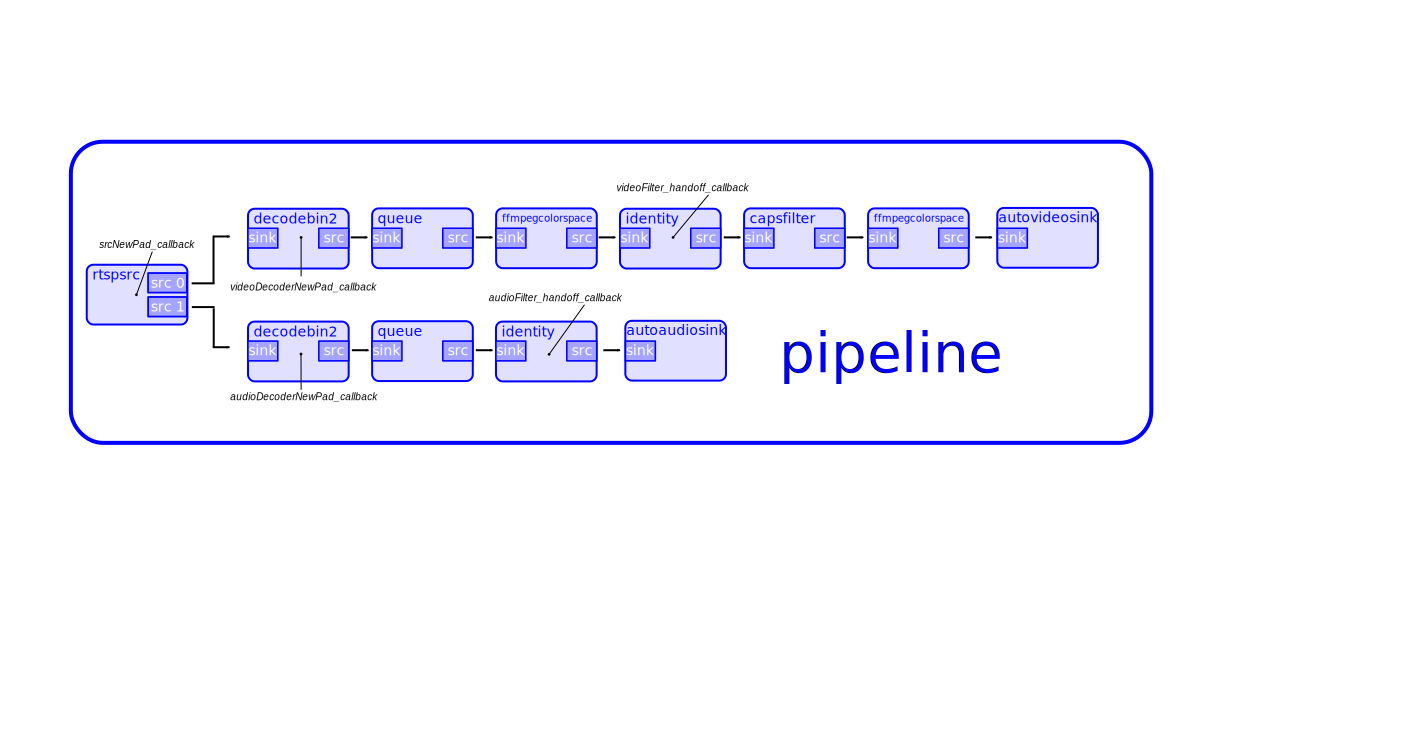
\includegraphics[width=1\textwidth]{./imagenes/pipe.png}	
	\caption{Estructura de la linea de flujo en rovioStreaming.}
\label{pipeline}
\end{figure}

\begin{figure}

  \lstset{language=c++}
  \lstset{commentstyle=\textit}
  \tiny
  \begin{lstlisting}[frame=trbl]{}
//------------------------------------------------------------------------------
class ADT_rovioAPI
{
 private:
	string uri;
	int sendCommand(const char *command) const;
	static int curlCallback(char *data, unsigned int size, unsigned int nmemb,
							 void *userdata);

 public:
 	rovioStreaming *streaming;
 	rovioSpeak *speak;
	void setHome() const;
	void goHome() const;
	void stop() const;
	void move(double angle, unsigned int speed) const;
	void rotate(double angle, unsigned int speed) const;
	void headUp() const;
	void headMiddle() const;
	void headDown() const;
	void light(int l) const;
	const char* getURI() const;
	ADT_rovioAPI(const char *_uri);
	~ADT_rovioAPI();
	
};
//------------------------------------------------------------------------------

  \end{lstlisting}
  \caption{ADT\_rovioAPI.h}
\end{figure}

\section{Ejemplo}
\label{ejemplo}
  Junto con el código de esta API se provee de un programa ejemplo para demostrar su funcionamiento. El programa ejemplo consiste en una interfaz gráfica en GTK+ y glade con la cual se accesa a las funciones del API.
% Para mayor información acerca de la programación con GTK+ se puede consultar \cite{GTKtutorial}.

  \subsection{Requisitos}
  Para compilar el programa ejemplo se requiere contar con el paquete \textbf{libgtk2.0-dev}. Las banderas de compilación se especifican en el archivo \textit{makefile} de este ejemplo. La interfaz gráfica se puede editar con el entrono de diseño Glade el cual es el paquete \textbf{glade-gnome}.

\section{Notas}
\label{notas}
El código fuente de esta API puede ser descargado en \href{http://www.aurea-dt.com/#rovioAPI}{nuestro sitio web}, en donde también se pueden reportar errores en el código fuente. Para reportar errores en este documento favor de escribir a \href{mailto:errata@aurea-dt.com}{errata@aurea-dt.com}.


% \bibliographystyle{plain}	% (uses file "plain.bst")
% \bibliography{/home/mchc/Aurea/CPP/Programs/ADTlib-0.0.1/Manual/ADTlib.bib}
\end{document}          
